\chapter{Summary}
\label{cha:summary}

Conducted experiments show a gap between JavaScript and C++ performance. Significant language design differences result in code that is often easier to write but also easier to abuse. Benchmarks show differences between 15\% and 100\% overhead for correctly designed JavaScript code and over 500\% for incorrect patterns.  Considering Moore's law stating that computers double speed every 18 months it safe to say that JavaScript is very close to being suitable for any type of development. Recent projects varying from server side solutions\footnote{http://nodejs.org/}\footnote{http://googlecreativelab.github.io/coder/} to hardware developer boards\footnote{http://www.espruino.com/} are proving it. From the perspective of game development, it is unlikely at the time of writing that AAA game may be created to run in browser. However, growing segments of casual, independent and social games are already targeting web as a platform.

\begin{figure}[h!]
  \caption{Game created with ImpactJS}
  \label{img:impactjs}
  \centering
	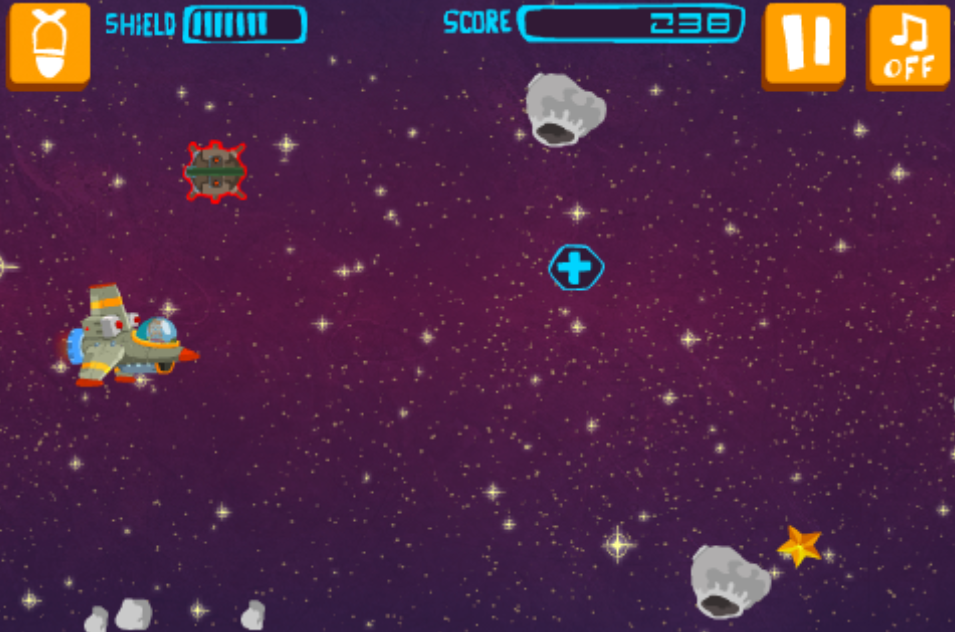
\includegraphics[width=12cm]{summary/impactjs.png}
\end{figure}

Multiple open-source and commercial game engines are created lately. Examples worth mentioning are ImpactJS\footnote{http://impactjs.com/}, Turbulenz\footnote{http://biz.turbulenz.com/turbulenz} and Isogenic Engine\footnote{http://www.isogenicengine.com/}.


\begin{figure}[h!]
  \caption{Game created with Isogenic Engine}
  \label{img:isogenic}
  \centering
	
\includegraphics[width=12cm]{summary/isogenic.png}
\end{figure}

Very important and growing sector are interactive 3D arts with two major targets - music videos and commercials. They are uniquely available only in browsers as a very viral extensions of normal marketing. One of the first occurrences of this technology was video for Rome music group: "3 dreams of black"\footnote{http://www.ro.me/}. Project allows to move the camera while animated 3D story is rendered alongside music. After movie is over user is allowed to create 3D models that are later incorporated into experiences of other people watching. This way interactions and social element are enabled in what used to be one-way transmission of art form. 

\begin{figure}[h!]
  \caption{Screenshot from "3 dreams of black"}
  \label{img:rome}
  \centering
	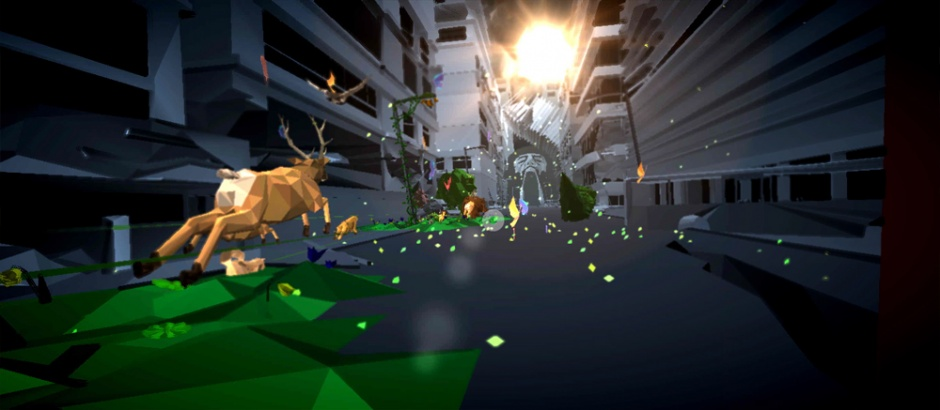
\includegraphics[width=12cm]{summary/rome.jpg}
\end{figure}

\section{Encountered environment limitations and recommended techniques}
\label{sec:limitations}

Conducted experiments show clear pattern regarding dynamic variable types in JavaScript. Whenever boxing and unboxing happens, JIT compilation is not able to properly optimise code and bring it up to performance of C++. This affects both simple variables and properties end is especially visible for numbers. Transitions between integer and floats are expensive while easy to overlook.

Types affect significantly also method calls cost. Keeping methods monomorphic in core parts of physics engine is very important. Additional cost of polymorphism of parameters is not only boxing and unboxing of parameters but also time spent of optimising and deoptimising compiled method which makes initial warmup of engine longer. Exporting well defined methods to be called from polymorphic ones is an easy workaround for this performance bottleneck.

Lastly, memory management proven to be one of the most important problems in JavaScript. Automated garbage collection connected with popular pattern of creating and returning of arrays is an important problem. Memory allocation of objects is also a bottleneck, but not very dissimilar to one in C++. As shown in second version of particle system, usage of object pools and changing architecture to avoid array creation are techniques that can be employed to fight with it. It is worth mentioning that while garbage collection always introduces some overhead it is reasonable to avoid it at all costs. Sphere collision system with octree partitioning is also introducing and destroying objects, but overhead is significantly smaller than gained speedup. Advice for memory operations is to avoid objects living only for a single frame i.e. temporary variables and helpers. Long living objects are in general unavoidable and should be used whenever suitable.

General advice for programming in JavaScript is to use techniques similar to those found in asm.js - keep types static, method calls monomorphic and work carefully with memory.

\section{Final thoughts}
\label{sec:final}

Original motivation for this work was a growing community around browser-based games. One of the main reasons why JavaScript gained such popularity in last years is clearly not a quality of maturity of language itself. Presented problems are topic of much discussion and, as mentioned in \ref{cha:overview} possibility of introducing better languages is explored.

While suffering from design issues, JavaScript provides a complete environment that makes development very easy for both beginner and advanced programmer. Two very important components of every application are provided out of the box - rendering system and networking in browser, designed for HTML pages to carry mainly text information is still suitable for gaming. Creation of simple 2D game is often a matter of few hundred lines of code responsible for transferring user input to positions of sprites defined in CSS. This is clearly visible during competitions like JS13kGames\footnote{http://js13kgames.com/} where all game assets and code have to be fitted into 13kB package.

Traditionally, games are often still sold in physical boxes and some update system is always incorporated to patch any bugs appearing after initial release. Systems like Steam\footnote{http://store.steampowered.com/} are making this process easier but still suffer from necessity to install a game on hard drive.

Creating application that works in browser simplifies distribution significantly. All assets and code are downloaded each time user enters a website, so no update system is necessary - all users always play the newest version. Usually browser games are monetised differently than traditional titles. Playing basic version is usually free and earnings come from either ads or premium content. This is completely new approach, present also in MMO\footnote{Massive Multiplayer Online} games. It resulted in psychological research on leveraging compulsive behaviours to maximise profits\footnote{http://www.emcneill.com/exploitative-game-design-beyond-the-f2p-debate/}.

Working in browser gives access to all social network of user, so incorporation of Twitter or Facebook based features is very simple - which boosts promotion of game. It also enables, morally questionable, target of people not able to install games on company issued computer. Disallowing games in browsers is far more complicated task for administrator, similar to blocking ads or mature content.

Lastly, web is better suited to run easily on all platforms. Browser is a layer of abstraction that makes transparent for application, whether it runs on any traditional operating system, gaming console or mobile device. Of course  performance and screen size should be taken under consideration, but ability to write one codebase that runs on multiple devices led already to projects that package JavaScript applications as native ones\footnote{http://phonegap.com/}, greatly reducing development costs for growing variety of phones and tablets.

Conducted tests show that while gap between JavaScript and native application exists and is not insignificant, there is a lot of potential in such approach. It is expected, that with growing community and interest from game industry new games will be released on browser within few years. Performance issues may prevent works on AAA titles, but companies focused more on social aspect of games and new trends in monetisation may create games targeted for different users. With capabilities of browsers equal to having 18 months older machine, less graphically demanding titles like The Sims or World or Warcraft may certainly be ported to run in JavaScript.

